\documentclass[10pt,a4paper]{amsart}
\usepackage[margin=19mm]{geometry}
\usepackage{amsmath,amssymb,mathtools}
\usepackage[scr=rsfs,cal=euler]{mathalfa}
\usepackage{xfrac}
\usepackage[unicode,hidelinks,bookmarks=false]{hyperref}
\newcommand{\ie}{i.e.\ }
\newcommand{\cf}{cf.\ }
\newcommand{\resp}{respectively\ }
\newcommand{\Subsection}{\subsection}
\providecommand{\nobreakdash}{\nobreak\hbox{-}}
\setlength{\emergencystretch}{2em}
\multlinegap0pt
\usepackage{tikz}
\usepackage{enumerate}
\usepackage{amssymb}
\usepackage{stackengine}
\newtheorem{lem}{Lemma}
\newtheorem{thm}{Theorem}
\newtheorem{claim}{Claim}
\title{Adjacent vertex distinguishing total chromatic number of graph products}
\author{Amitayu Banerjee, Jayabalan Geetha, Kanagasabapathi Somasundaram}
\date{Source: arXiv:2609.03411v1 (CC BY 4.0)}
\begin{document}
\maketitle

\noindent\emph{Source and licence.} Adjacent vertex distinguishing total chromatic number of graph products. Version arXiv:2609.03411v1 (CC BY 4.0), distributed by arXiv under the Creative Commons Attribution 4.0 International licence, http://creativecommons.org/licenses/by/4.0/, as recorded in the arXiv licence metadata for this exact version and shown on the abstract page https://arxiv.org/abs/2609.03411v1. Full licence notice: \texttt{licenses/arxiv-2609.03411-CC-BY-4.0.txt}.\par\smallskip

\noindent\textit{Editorial scope.} Counted unit: the article's thm 8.1 (source0.tex lines 1355--1364). The article's complete original proof of it is delivered with it (source0.tex lines 1366--1619, one \texttt{proof} environment of 254 lines). No mathematics is written, repaired or re-derived: the statement and the proof are the article's own lines, in the article's own notation, and no retained line is substituted or re-flowed.  Retained uncounted as the source-local context the proof needs: lines 241--248.  Nothing was omitted from any retained span, so the package carries no omission record.  No retained line contains a citation, so the wrapper carries no bibliography and no bibliography entry.  The retained lines contain the article's own diagram code, which the wrapper typesets with the standard tikz packages; no image file is delivered and the package declares no asset dependency.  Editorial formatting only, in addition: an AMS \texttt{amsart} preamble that restates the article's own declarations and macros used by the retained lines, namely the environments \texttt{lem}, \texttt{thm}, \texttt{claim} on separate counters, together with the standard packages those lines need.  The retained environments print in this document as Lemma 1, Theorem 1, Claim 1 in order of appearance, whereas the article prints the same items with the numbering of its own full document.  The complete native source of the article as distributed in the arXiv e-print for this exact version is bundled unchanged as \texttt{sources/209296/source0.tex}.
\begin{lem}\label{Lemma 2.2}
    {\em Fix $n>2$. Let $M = [m_{i,j}]$ be a Latin square where $m_{i,j} \equiv (i + j)-1 \pmod{n}, 1 \leq m_{i,j} \leq n$, for $1 \leq i, j \leq n$. If $k,l<n$, and $M'$ is the submatrix of $M$ consisting of the first $k$ rows and the first $l$ columns of $M$, then 
    \begin{enumerate}
        \item no two rows of $M'$ contain the same set of entries,
        \item no two columns of $M'$ contain the same set of entries.
    \end{enumerate}
    }
\end{lem}

\begin{thm}\label{Theorem 8.1}
    {\em Let $G_1$ and $G_2$ be graphs of order $m$ and $n$ respectively such that
    \begin{enumerate}
        \item $m>n+1$,
        \item $\Delta(G_2)\geq\Delta(G_1)$, and
        \item $G_2$ is a total colorable graph.
    \end{enumerate}
    Then, $G=G_1\blacktriangledown G_2$ satisfies the AVDTCC.    
    }
\end{thm}

\begin{proof}
Let $H_1$ be the first copy of $G_1 \vee G_2$ and $H_2$ be the second copy of $G_1 \vee G_2$. Let $G_1'$ and $G_2'$ denote the copies of $G_1$ and $G_2$ in $H_2$. 
Suppose $V(G_1)=\{u_1,...,u_m\}$, $V(G_2)=\{v_1,...,v_n\}$, $V(G'_1)=\{u'_1,...,u'_m\}$ and $V(G'_2)=\{v'_1,...,v'_n\}$ be the set of vertices of $G_1, G_2, G'_1$ and $G'_2$ respectively (see Fig. \ref{Figure 6}). 
We note that $\Delta(G)=\max\{\Delta(G_1)+n,\ \Delta(G_2)+m+1\}=\Delta(G_2)+m+1.$

\begin{figure}[ht]
    \centering
    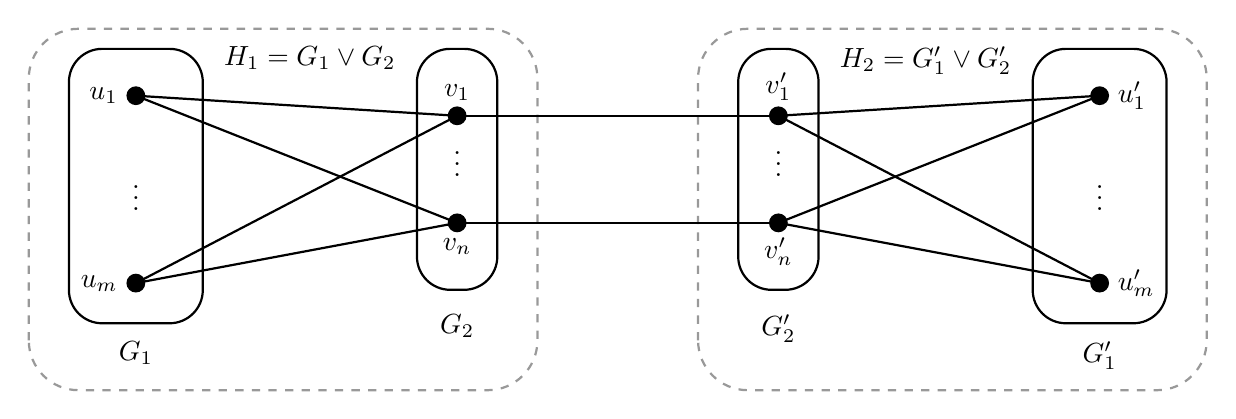
\begin{tikzpicture}[scale=1.7]

        % ==================================================
        % 1. OUTER GROUPING CONTAINERS
        % ==================================================
        \draw[thick, dashed, gray!80, rounded corners=18pt]
            (-4.4,-1.5) rectangle (-0.6,1.2);

        \draw[thick, dashed, gray!80, rounded corners=18pt]
            (0.6,-1.5) rectangle (4.4,1.2);

        % ==================================================
        % 2. VERTICAL CAPSULES
        % ==================================================
        % G1
        \draw[thick, rounded corners=12pt]
            (-4.1,-1) rectangle (-3.1,1.05);
        \node[below=3pt] at (-3.6,-1) {$G_1$};

        \node[below=3pt] at (-2.3,1.2) {$H_1=G_1\vee G_2$};

        % G2
        \draw[thick, rounded corners=12pt]
            (-1.5,-0.75) rectangle (-0.9,1.05);
        \node[below=3pt] at (-1.2,-0.8) {$G_2$};

        % G2'
        \draw[thick, rounded corners=12pt]
            (0.9,-0.75) rectangle (1.5,1.05);
        \node[below=3pt] at (1.2,-0.8) {$G_2'$};
        \node[below=3pt] at (2.3,1.2) {$H_2=G'_1\vee G'_2$};

        % G1'
        \draw[thick, rounded corners=12pt]
            (3.1,-1) rectangle (4.1,1.05);
        \node[below=3pt] at (3.6,-1) {$G_1'$};

        % ==================================================
        % 3. VERTICES
        % ==================================================
        % G1
        \fill (-3.6,0.7) circle (2pt) coordinate (U1);
        \fill (-3.6,-0.7) circle (2pt) coordinate (Um);
        \node[left=3pt] at (U1) {$u_1$};
        \node[left=3pt] at (Um) {$u_m$};
        \node at (-3.6,0) {$\vdots$};

        % G2
        \fill (-1.2,0.55) circle (2pt) coordinate (V1);
        \fill (-1.2,-0.25) circle (2pt) coordinate (Vn);
        \node[above=2pt] at (V1) {$v_1$};
        \node[below=2pt] at (Vn) {$v_n$};
        \node at (-1.2,0.25) {$\vdots$};

        % G2'
        \fill (1.2,0.55) circle (2pt) coordinate (V1p);
        \fill (1.2,-0.25) circle (2pt) coordinate (Vnp);
        \node[above=2pt] at (V1p) {$v_1'$};
        \node[below=2pt] at (Vnp) {$v_n'$};
        \node at (1.2,0.25) {$\vdots$};

        % G1'
        \fill (3.6,0.7) circle (2pt) coordinate (U1p);
        \fill (3.6,-0.7) circle (2pt) coordinate (Ump);
        \node[right=3pt] at (U1p) {$u_1'$};
        \node[right=3pt] at (Ump) {$u_m'$};
        \node at (3.6,0) {$\vdots$};

        % ==================================================
        % 4. CROSS EDGES
        % ==================================================
        % G1 to G2
        \draw[thick] (U1) -- (V1);
        \draw[thick] (U1) -- (Vn);
        \draw[thick] (Um) -- (V1);
        \draw[thick] (Um) -- (Vn);

        % G2 to G2'
        \draw[thick] (V1) -- (V1p);
        \draw[thick] (Vn) -- (Vnp);

        % G2' to G1'
        \draw[thick] (V1p) -- (U1p);
        \draw[thick] (V1p) -- (Ump);
        \draw[thick] (Vnp) -- (U1p);
        \draw[thick] (Vnp) -- (Ump);

    \end{tikzpicture}
    \caption{The Indu-Bala product $G_1 \blacktriangledown G_2$.}
    \label{Figure 6}
\end{figure}

Consider a Latin square $M=[m_{i,j}]$ of order $t=m+1$ as in Lemma \ref{Lemma 2.2}. 
Let $M'$ consists of the first $m$ rows and $n+1$ columns of $M$.
We define
    \[
    g_1(x)=
    \begin{cases}
    m_{i,j}, & x=u_i v_j, 1\leq i\leq m, 1\leq j\leq n\\[2mm]
    m_{i,n+1}, & x=u_i, 1\leq i\leq m.
    \end{cases}
    \]
Consider the complete bipartite graph $B(H_1)$ with bipartitions $V(G_1)$ and $V(G_2)$, which is a subgraph of $H_1$. Let $C=\{1,...,m+1\}$ be the set of entries of $M$. 

\begin{claim}\label{Claim 8}
{\em The following holds:
\begin{enumerate}
    \item No two adjacent edges in $B(H_1)$ receive the same color. 
    \item Each vertex $u_i$ receives a color distinct from its incident edges in $B(H_1)$. 
    \item %If $D_{B(H_1)}(u)$ is the set of colors on the edges incident with $u$ in $B(H_1)$, then
    $D_{B(H_1)}(v_i)\neq D_{B(H_1)}(v_j)$
    and
    $C_{B(H_1)}(u_i)\neq C_{B(H_1)}(u_j)$ for any  $i\neq j$.
\end{enumerate}
}
\end{claim}

\textit{Proof:}
(1) and (2) hold since each element of $M$
occurs exactly once in each row and exactly once in each column of $M$ and (3) follows from Lemma \ref{Lemma 2.2}.

Let $D=\{m+2, m+3,...,m+\Delta(G_{2})+3\}$ be a set of $\Delta(G_2)+2$ colors.
Since $G_2$ satisfies the TCC, there exists a proper total coloring $g_2:V(G_2)\cup E(G_2)\rightarrow D$ of $G_2$.
Let $g_3:E(G_1)\rightarrow D$ be a proper edge coloring of $G_1$. This is possible since $\chi'(G_1)\leq \Delta(G_1)+1<\Delta(G_2)+2$.\\
We define a total coloring
$g:V(H_1)\cup E(H_1)\rightarrow C\cup D$ by
\[
g(x)=
\begin{cases}
g_1(x), & \text{if } x\in V(G_1)\cup E(B(H_1)),\\
g_2(x), & \text{if } x\in V(G_2)\cup E(G_2),\\
g_3(x), & \text{if } x\in E(G_1).
\end{cases}
\]
Now, we color the elements of $H_2$.
Define $g_1'$ using the elements of $M'$ as follows:
\[
g_1'(x)=
\begin{cases}
m_{i,j+1}, & x=u_i'v_j', 1\leq i\leq m, 1\leq j\leq n\\[2mm]
m_{i,n+2}, & x=u_i', 1\leq i\leq m.
\end{cases}
\]
Let $\sigma$ be a cyclic permutation of all the colors in $D$, so that $\sigma(d)\neq d$ for any $d\in D$. 
Let $g_2':V(G_2')\cup E(G_2')\rightarrow D$ be the total coloring of $G_2'$  defined by 
\[
g_2'(x)=
\begin{cases}
\sigma(g_2(v_i)), & \text{if }x=v'_i,\\[1mm]
\sigma(g_2(v_iv_j)), & \text{if }x=v_i'v_j'.
\end{cases}
\]
%Let $g_2':V(G_2')\cup E(G_2')\rightarrow D$ be the total coloring of $G_2'$  defined by 
%\begin{center}
%    $g_2'(x):=g_2(x)+1
%\pmod{\Delta(G_2)+2}$.
%\end{center}
The definition of $g_2'$ ensures that $g_2'(v'_i)\neq g_2(v_i)$ for each $v_i\in V(G_2)$ and $v'_i\in V(G'_2)$ where $1\leq i\leq n$.
Similar to the coloring $g_3$, let $g_3': E(G_1')\rightarrow D$ be a proper edge coloring  of $G_1'$. 
We define a total coloring
$g':V(H_2)\cup E(H_2)\rightarrow C\cup D$ by
\[
g'(x)=
\begin{cases}
g'_1(x), & \text{if } x\in V(G'_1)\cup E(B(H_2)),\\
g'_2(x), & \text{if } x\in V(G'_2)\cup E(G'_2),\\
g'_3(x), & \text{if } x\in E(G'_1).
\end{cases}
\]
We use a new color $c$ to color all the edges $\{v_iv_i':1\le i\leq n\}$.\\
Define a total coloring $h : E(G)\cup V(G)\rightarrow C \cup D \cup \{c\}$ of $G$ by
\[h(x)=
\begin{cases}
g(x), & \text{if } x \text{ is an element of } H_1,\\[1ex]
g'(x), & \text{if } x \text{ is an element of } H_2,\\[1ex]
c, & \text{if } x \in \{v_iv_i' : 1 \leq i \leq n\,\}.
\end{cases}
\]
It is clear that \(h\) is a proper total coloring of $G$ and $|C\cup D\cup \{c\}|=\left(\Delta(G_2)+m+1\right)+3$.

\begin{claim}\label{Claim 9}
{\em $D_{B(H_1)}(v_j)\neq D_{B(H_2)}(v_j')$ for each $1\leq j\leq n$.}
\end{claim}

\textit{Proof:}
The definition of $g_1'$ ensures that if $B(H_i)$ is the bipartite induced subgraph of $H_i$ $(i=1,2)$, then $D_{B(H_1)}(v_j)=\{m_{1,j},...,m_{m,j}\}\neq \{m_{1,j+1},...,m_{m,j+1}\}= D_{B(H_2)}(v_j')$ by Lemma \ref{Lemma 2.2}.    

\begin{claim}\label{Claim 10}
{\em The coloring $h$ is an AVD-total coloring of $G$.}
\end{claim}

\textit{Proof:}
Let $uv \in E(G)$ be an arbitrary edge. 

\textbf{Case (i):}
Suppose $u=u_i$ and $v=u_j$ such that $uv\in E(G_1)$.
Then for $x\in \{i,j\}$,
\begin{center}
    $C_G(u_x)=C_{B(H_1)}(u_x)\cup D_{G_1}(u_x)$,
\end{center}
where $C_{B(H_1)}(u_x)\subseteq C$ and $D_{G_1}(u_x)\subseteq D$. Moreover, $C_{B(H_1)}(u_i)\neq C_{B(H_1)}(u_j)$ by Lemma \ref{Lemma 2.2}.
Since $C\cap D=\emptyset$, we obtain $C_{G}(u)=C_G(u_i)\neq C_G(u_j)=C_{G}(v)$.
Similarly, if $uv\in E(G_1')$ then $C_G(u)\neq C_G(v)$.

\textbf{Case (ii):} 
Suppose $u=u_i$ and $v=v_j$ such that $uv\in E(H_1)$. 
Then $|C_G(u_i)\cap C|=n+1$ and
$|C_G(v_j)\cap C|=m$.
Since $m>n+1$, we obtain
$C_G(u_i)\neq C_G(v_j)$.
Similarly, if $u=u'_i$ and $v=v'_j$ such that $u'_iv'_j\in E(H_2)$, then $C_G(u'_i)\neq C_{G}(v'_j)$.     

\textbf{Case (iii):} 
Let $u=v_i, v=v_j$ such that $v_iv_j\in E(G_2)$. The following holds:
\begin{enumerate}
    \item $D_{B(H_1)}(v_i)\neq D_{B(H_1)}(v_j)$ by Lemma \ref{Lemma 2.2},
    
    \item $C_{G}(v_x)=D_{B(H_1)}(v_x)\cup h(v_xv_x')\cup C_{G_2}(v_x)$ for $x\in \{i,j\}$, 
    
    \item $C 
    \cap
    \left\{
    h(v_xv_x')\cup C_{G_2}(v_x)
    \right\}
    =\emptyset$ and $D_{B(H_1)}(v_x)\subseteq C$ for $x\in \{i,j\}$.
\end{enumerate}
Thus, $C_{G}(v_i)\neq C_{G}(v_j)$.
Similarly, if $u=v'_i$, $v=v'_j$, and $uv\in E(G'_2)$ then $C_{G}(v'_i)\neq C_{G}(v'_j)$.

\textbf{Case (iv):}
Let $u=v_i$, $v=v_i'$ and $v_iv'_i\in E(G)$.
Then, the following holds:
\begin{enumerate}
    \item $D_{B(H_1)}(v_i) \neq D_{B(H_2)} (v'_i)$ by Claim \ref{Claim 9},
    
    \item $C_G(v_i)=D_{B(H_1)}(v_i)\cup h(v_i v_i') \cup C_{G_2}(v_i)$,
    
    \item $C_G(v'_i)=D_{B(H_2)}(v'_i)\cup h(v_i v_i') \cup C_{G'_2}(v'_i)$,
    
    \item $D_{B(H_1)}(v_i), D_{B(H_2)}(v'_i)\subseteq C$,

    \item 
    $C \cap \left\{ h(v_i v_i') \cup C_{G_2}(v_i) \right\} = \emptyset$ and $C \cap \left\{ h(v_i v_i') \cup C_{G'_2}(v'_i) \right\} = \emptyset$.
\end{enumerate}

Consequently, $C_G(v_i) \neq C_G(v_i')$. 
\end{proof}

\end{document}
